\chapter{Experiments} \label{chap:experiments}

In this chapter, we explain the setup of our experiments, describe how we measure the performance of different methods, and present the results. All experiments were performed using either the AMD EPYC 9454 or the AMD EPYC 9474F CPUs.

\section{Experiment 2: Optimization}

In the second experiment, we compare different optimization methods on datasets B--F. The goal is to find if some method is superior to others or if the ideal method is dataset-dependent. We also want to see how much we can improve from the starting solutions.

\subsection*{Methodology}

We compare the three previously mentioned optimization methods: \textit{\textbf{genetic algorithm}}, \textit{\textbf{hill climbing}} and \textit{\textbf{simulated annealing}}. For each dataset and method, 10 runs with different seeds were performed and averaged to obtain reliable results. ...

\newpage

\begin{figure}[h]
    \centering
    % 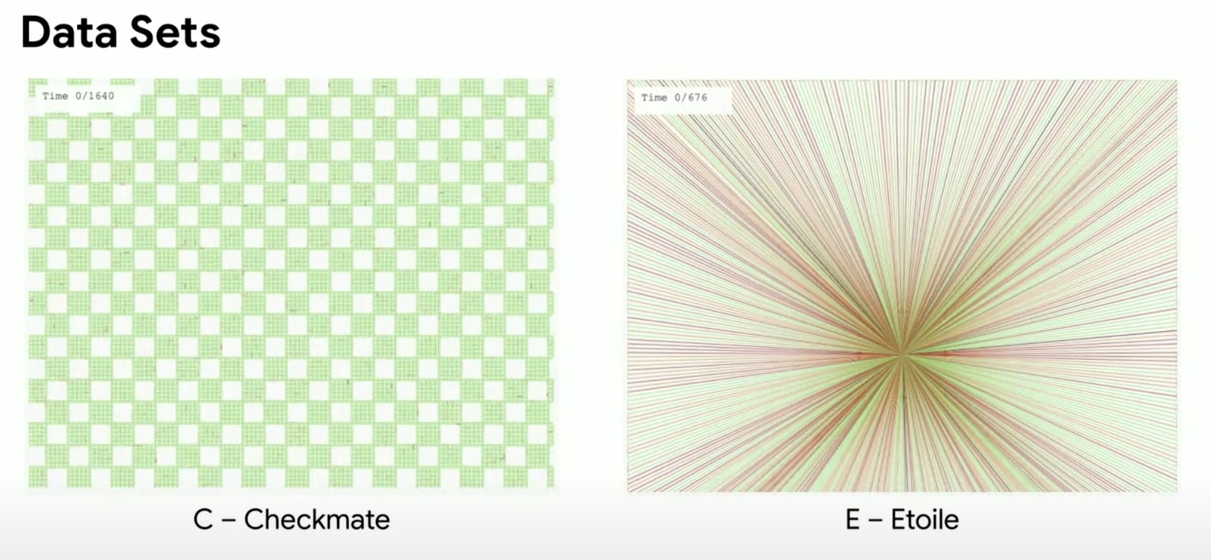
\includegraphics[width=\linewidth]{img/screenshots/hashcode_datasets_c_e.png}
    % 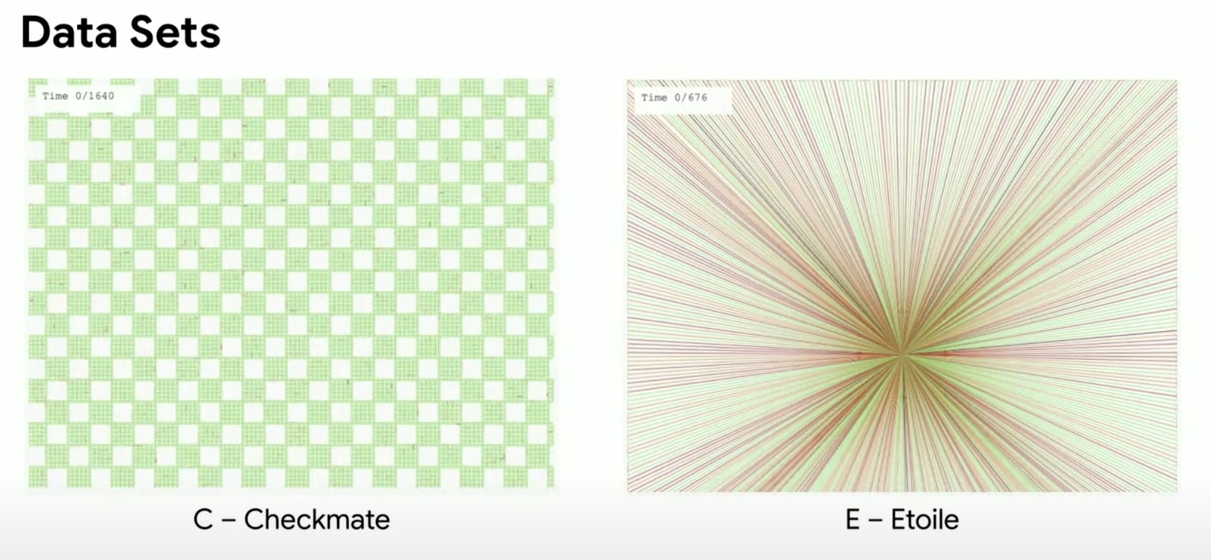
\includegraphics[width=.8\linewidth]{img/screenshots/hashcode_datasets_c_e.png}
    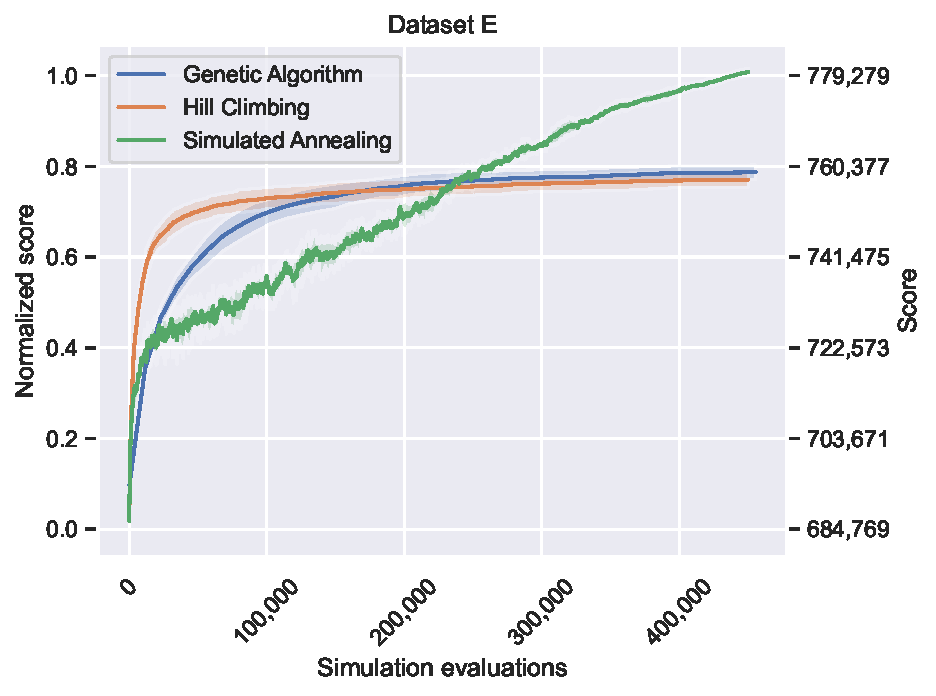
\includegraphics[width=\linewidth]{img/experiments/e_Genetic Algorithm_Hill Climbing_Simulated Annealing.pdf}
    \caption[Results for dataset E]{
        Results for dataset E.
    }
    \label{fig:dataset_e_experiment}
\end{figure}

\begin{table}[h]
\centering\footnotesize\sf
\begin{tabular}{lccc}
\toprule
& Normalized Score & Score & Time \\
\midrule
\textcolor{myblue}{\textbf{Genetic Algorithm}} & 87.82 & 767,768 & 0:06:43 \\
\textcolor{myorange}{\textbf{Hill Climbing}} & 86.79 & 766,798 & 0:06:58 \\
\textcolor{mygreen}{\textbf{Simulated Annealing}} & \textbf{101.08} & 780,299 & 0:07:03 \\
\bottomrule
\end{tabular}
%}{  % uncomment if you use the \floatbox (as above), erase otherwise
\caption[Results for dataset E]{Results for dataset E.}
%}  % uncomment if you use the \floatbox
\label{tab:dataset_e_results}
\end{table}

\newpage

\begin{figure}[h]
    \centering
    % 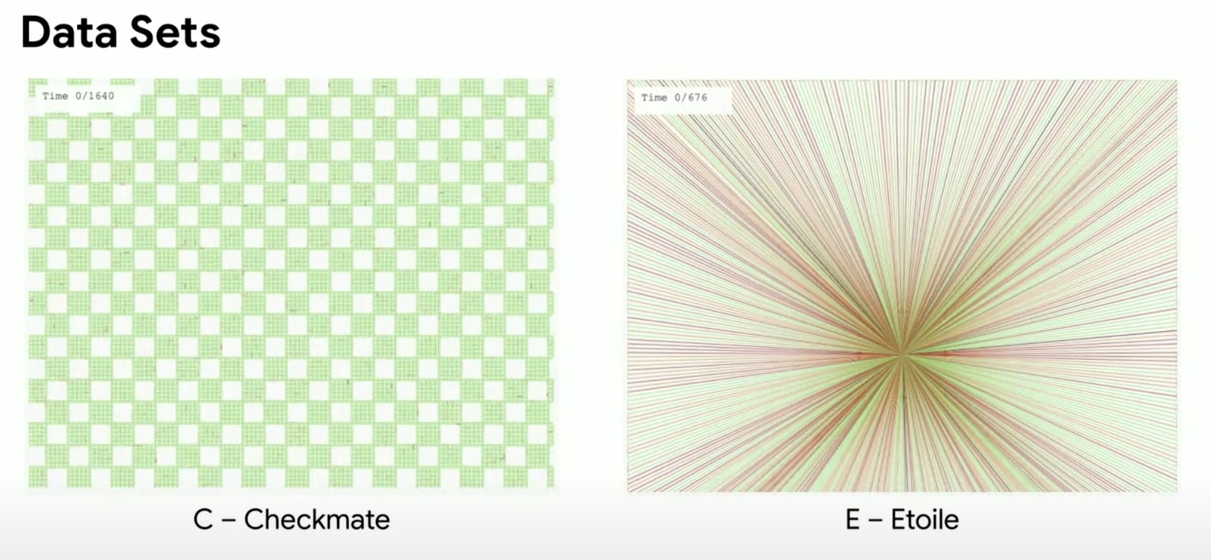
\includegraphics[width=\linewidth]{img/screenshots/hashcode_datasets_c_e.png}
    % 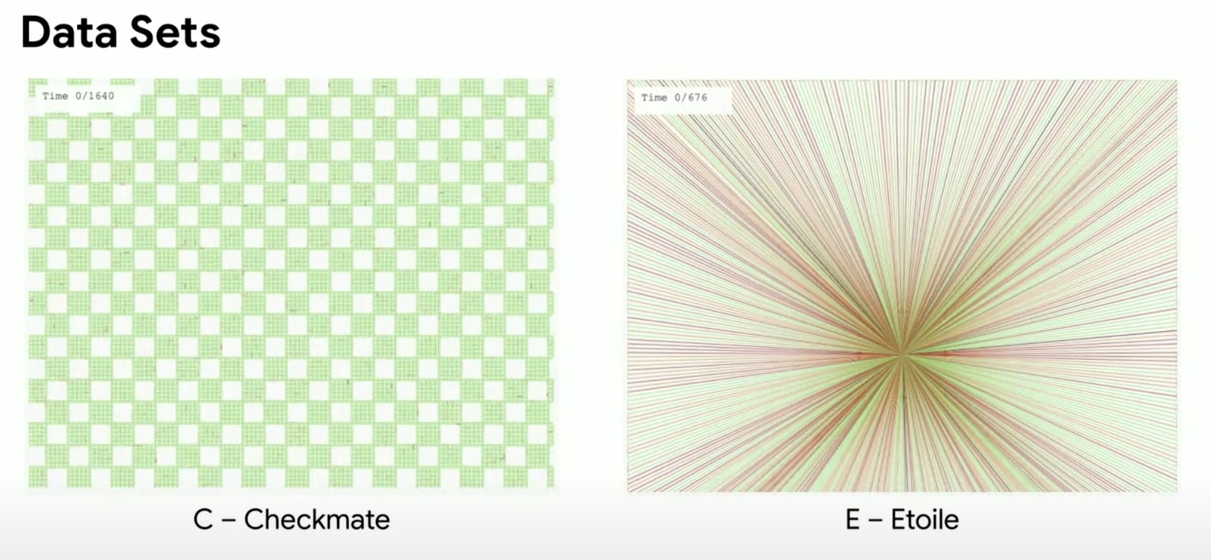
\includegraphics[width=.8\linewidth]{img/screenshots/hashcode_datasets_c_e.png}
    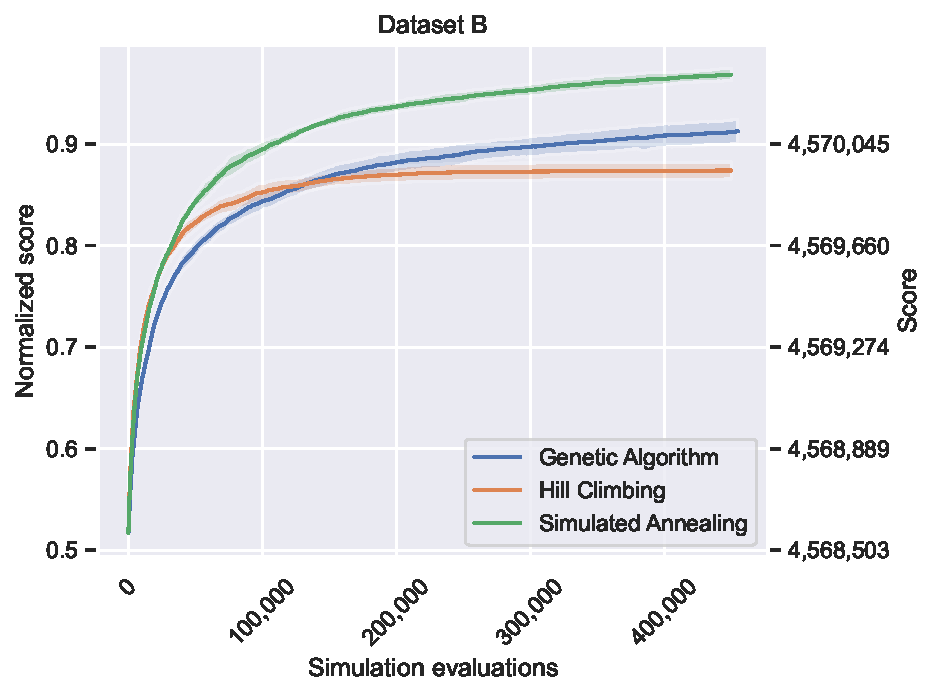
\includegraphics[width=\linewidth]{img/experiments/b_Genetic Algorithm_Hill Climbing_Simulated Annealing.pdf}
    \caption[Results for dataset B]{
        Results for dataset B.
    }
    \label{fig:dataset_b_experiment}
\end{figure}

\begin{table}[h]
\centering\footnotesize\sf
\begin{tabular}{lccc}
\toprule
& Normalized Score & Score & Time \\
\midrule
\textcolor{myblue}{\textbf{Genetic Algorithm}} & 91.29 & 4,570,095 & 0:42:15 \\
\textcolor{myorange}{\textbf{Hill Climbing}} & 87.40 & 4,569,945 & 0:55:35 \\
\textcolor{mygreen}{\textbf{Simulated Annealing}} & \textbf{96.84} & 4,570,309 & 0:55:12 \\
\bottomrule
\end{tabular}
%}{  % uncomment if you use the \floatbox (as above), erase otherwise
\caption[Results for dataset B]{Results for dataset B.}
%}  % uncomment if you use the \floatbox
\label{tab:dataset_b_results}
\end{table}

\newpage

\begin{figure}[h]
    \centering
    % 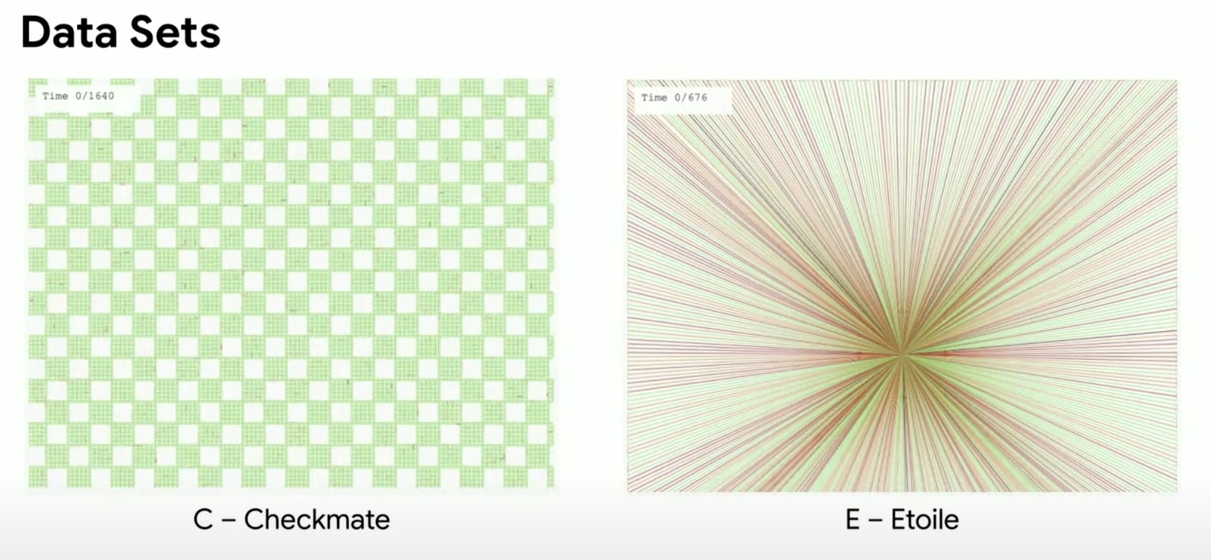
\includegraphics[width=\linewidth]{img/screenshots/hashcode_datasets_c_e.png}
    % 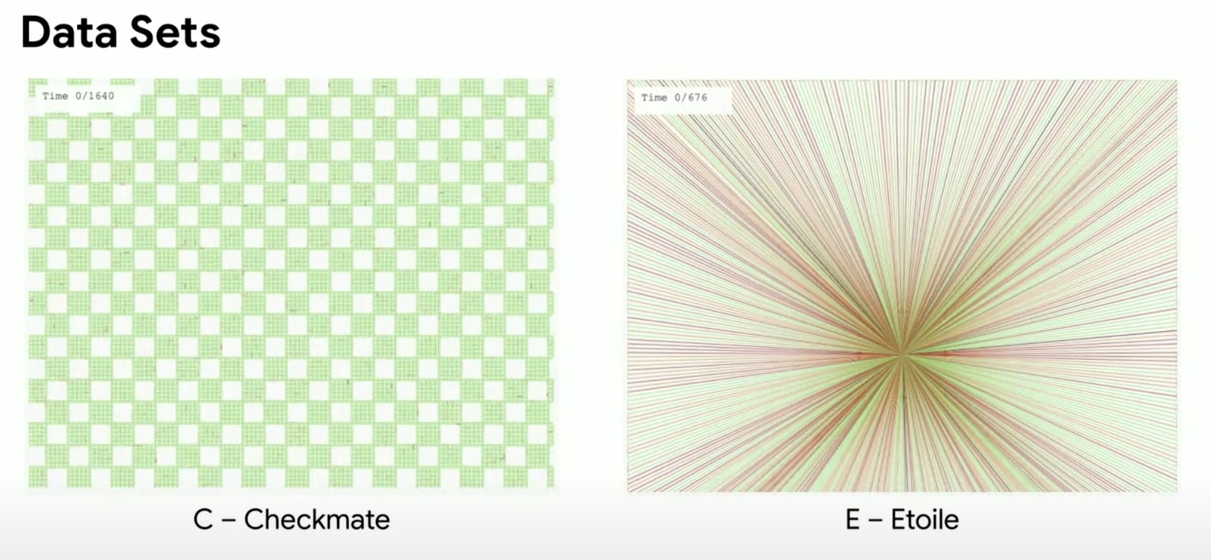
\includegraphics[width=.8\linewidth]{img/screenshots/hashcode_datasets_c_e.png}
    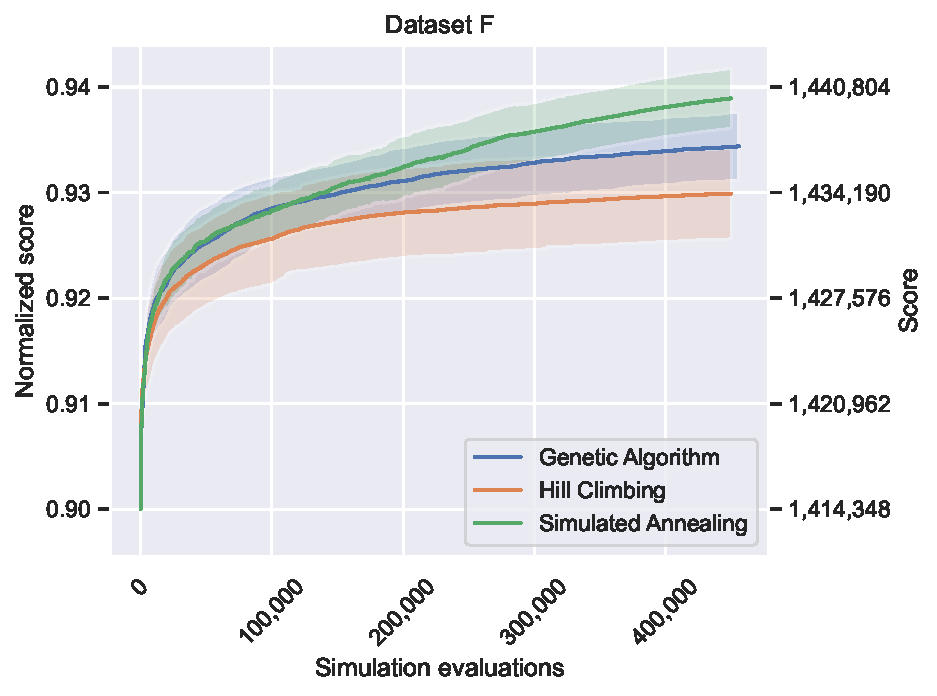
\includegraphics[width=\linewidth]{img/experiments/f_Genetic Algorithm_Hill Climbing_Simulated Annealing.pdf}
    \caption[Results for dataset F]{
        Results for dataset F.
    }
    \label{fig:dataset_f_experiment}
\end{figure}

\begin{table}[h]
\centering\footnotesize\sf
\begin{tabular}{lccc}
\toprule
& Normalized Score & Score & Time \\
\midrule
\textcolor{myblue}{\textbf{Genetic Algorithm}} & 93.44 & 1,437,086 & 1:47:39 \\
\textcolor{myorange}{\textbf{Hill Climbing}} & 92.99 & 1,434,129 & 2:38:58 \\
\textcolor{mygreen}{\textbf{Simulated Annealing}} & \textbf{93.89} & 1,440,097 & 2:23:53 \\
\bottomrule
\end{tabular}
%}{  % uncomment if you use the \floatbox (as above), erase otherwise
\caption[Results for dataset F]{Results for dataset F.}
%}  % uncomment if you use the \floatbox
\label{tab:dataset_f_results}
\end{table}

\newpage

\begin{figure}
    \centering
    % 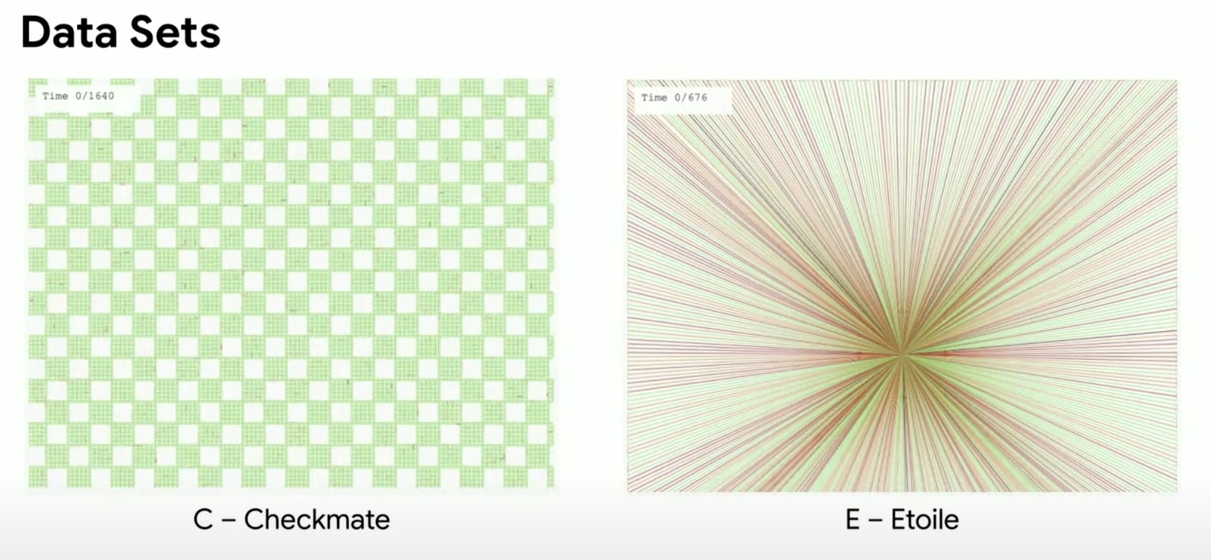
\includegraphics[width=\linewidth]{img/screenshots/hashcode_datasets_c_e.png}
    % 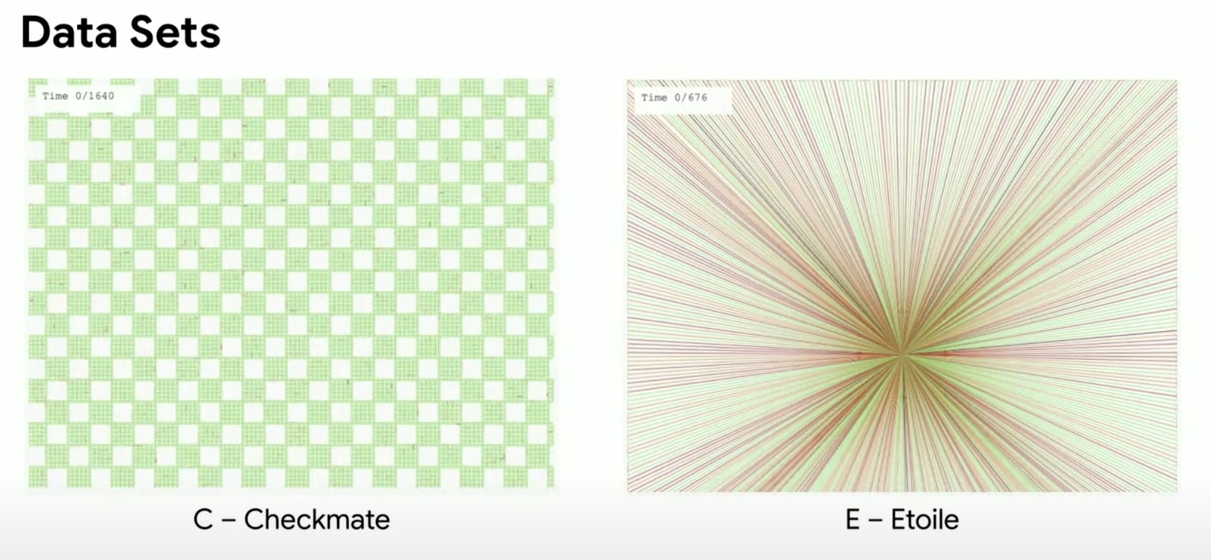
\includegraphics[width=.8\linewidth]{img/screenshots/hashcode_datasets_c_e.png}
    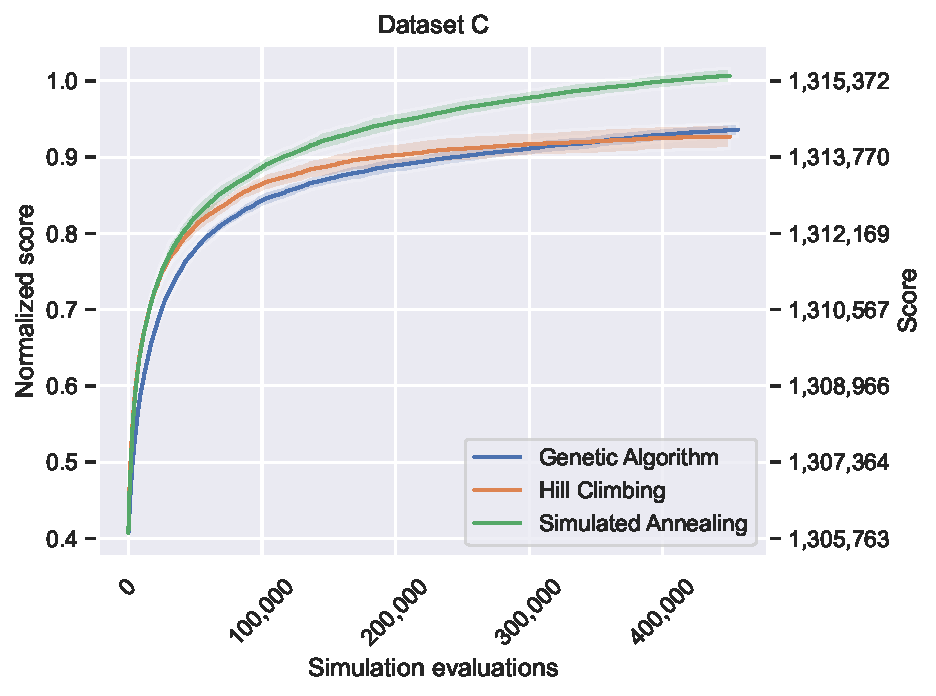
\includegraphics[width=\linewidth]{img/experiments/c_Genetic Algorithm_Hill Climbing_Simulated Annealing.pdf}
    \caption[Results for dataset C]{
        Results for dataset C.
    }
    \label{fig:dataset_c_experiment}
\end{figure}

\begin{table}[h]
\centering\footnotesize\sf
\begin{tabular}{lccc}
\toprule
& Normalized Score & Score & Time \\
\midrule
\textcolor{myblue}{\textbf{Genetic Algorithm}} & 93.60 & 1,314,347 & 1:54:28 \\
\textcolor{myorange}{\textbf{Hill Climbing}} & 92.68 & 1,314,200 & 3:18:31 \\
\textcolor{mygreen}{\textbf{Simulated Annealing}} & \textbf{100.65} & 1,315,476 & 2:58:44 \\
\bottomrule
\end{tabular}
%}{  % uncomment if you use the \floatbox (as above), erase otherwise
\caption[Results for dataset C]{Results for dataset C.}
%}  % uncomment if you use the \floatbox
\label{tab:dataset_c_results}
\end{table}

\newpage

\begin{figure}
    \centering
    % 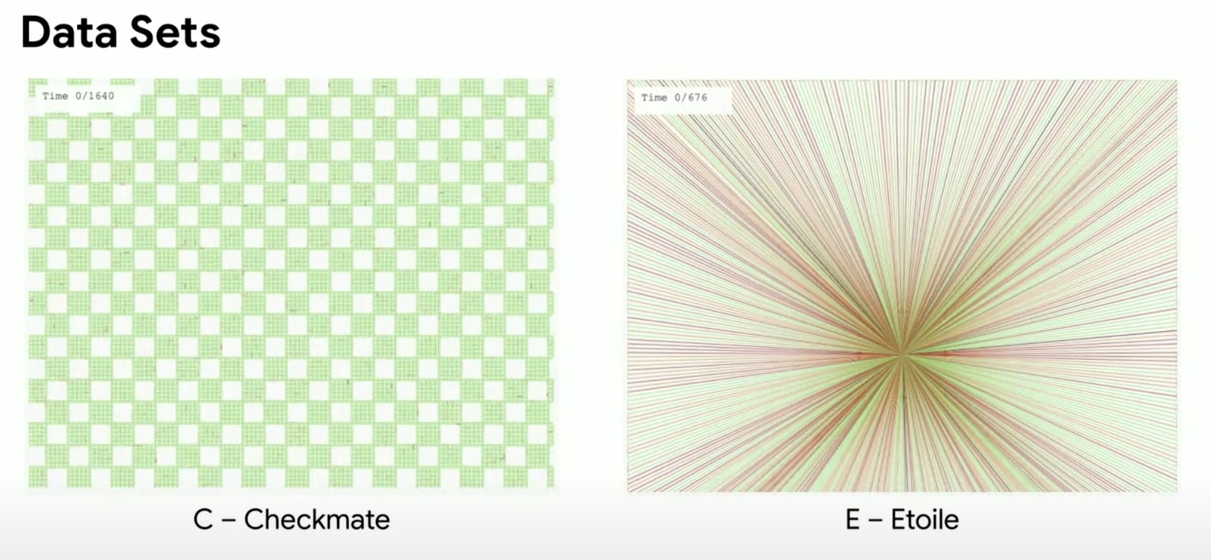
\includegraphics[width=\linewidth]{img/screenshots/hashcode_datasets_c_e.png}
    % 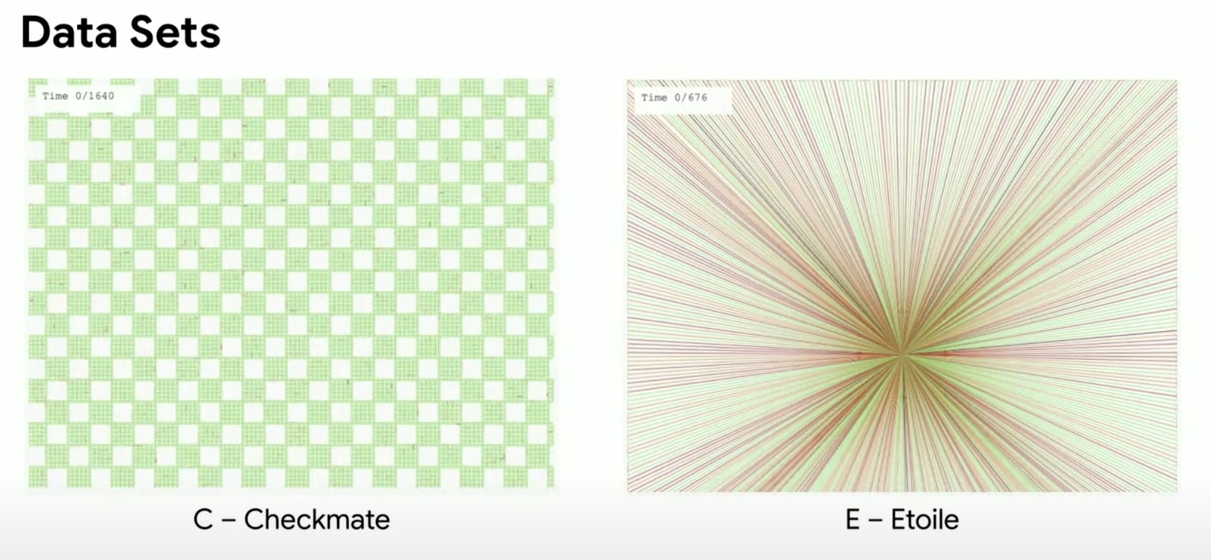
\includegraphics[width=.8\linewidth]{img/screenshots/hashcode_datasets_c_e.png}
    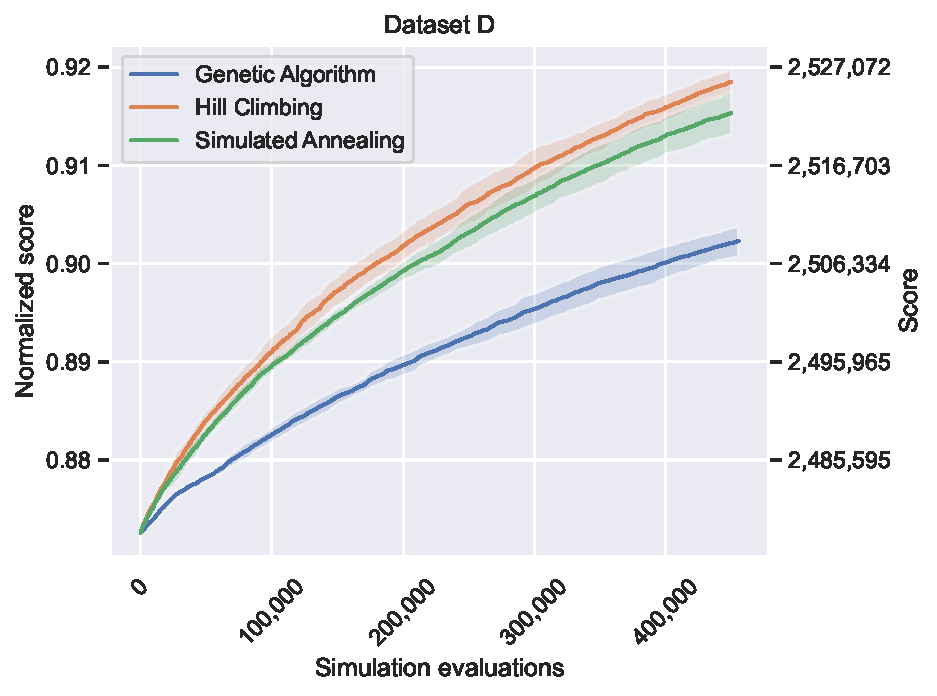
\includegraphics[width=\linewidth]{img/experiments/d_Genetic Algorithm_Hill Climbing_Simulated Annealing.pdf}
    \caption[Results for dataset D]{
        Results for dataset D.
    }
    \label{fig:dataset_d_experiment}
\end{figure}

\begin{table}[h]
\centering\footnotesize\sf
\begin{tabular}{lccc}
\toprule
& Normalized Score & Score & Time \\
\midrule
\textcolor{myblue}{\textbf{Genetic Algorithm}} & 90.23 & 2,508,730 & 9:12:47 \\
\textcolor{myorange}{\textbf{Hill Climbing}} & \textbf{91.85} & 2,525,531 & 20:14:01 \\
\textcolor{mygreen}{\textbf{Simulated Annealing}} & 91.53 & 2,522,204 & 22:17:16 \\
\bottomrule
\end{tabular}
%}{  % uncomment if you use the \floatbox (as above), erase otherwise
\caption[Results for dataset D]{Results for dataset D.}
%}  % uncomment if you use the \floatbox
\label{tab:dataset_d_results}
\end{table}

% \begin{table}[b!]

% \centering
% %% Tabulka používá následující balíčky:
% %%   - booktabs (\toprule, \midrule, \bottomrule)
% %%   - dcolumn (typ sloupce D: vycentrovaná čísla zarovnaná na
% %%     desetinnou čárku
% %%     Všimněte si, že ve zdrojovém kódu jsou desetinné tečky, ale
% %%     tisknou se čárky.
% %% Dále používáme příkazy \pulrad a \mc definované v makra.tex

% \begin{tabular}{l@{\hspace{1.5cm}}D{.}{,}{3.2}D{.}{,}{1.2}D{.}{,}{2.3}}
% \toprule
%  & \mc{} & \mc{\textbf{Směrod.}} & \mc{} \\
% \pulrad{\textbf{Efekt}} & \mc{\pulrad{\textbf{Odhad}}} & \mc{\textbf{chyba}$^a$} &
% \mc{\pulrad{\textbf{P-hodnota}}} \\
% \midrule
% Abs. člen     & -10.01 & 1.01 & \mc{---} \\
% Pohlaví (muž) & 9.89   & 5.98 & 0.098 \\
% Výška (cm)    & 0.78   & 0.12 & <0.001 \\
% \bottomrule
% \multicolumn{4}{l}{\footnotesize \textit{Pozn:}
% $^a$ Směrodatná chyba odhadu metodou Monte Carlo.}
% \end{tabular}

% \caption{Maximálně věrohodné odhady v~modelu M.}\label{tab03:Nejaka}

% \end{table}

\begin{table}
% uncomment the following line if you use the fitted top captions for tables
% (see the \floatsetup[table] comments in `macros.tex`.
%\floatbox{table}[\FBwidth]{
\centering\footnotesize\sf
\begin{tabular}{llrl}
\toprule
Column A & Column 2 & Numbers & More \\
\midrule
Asd & QWERTY & 123123 & -- \\
Asd qsd 1sd & \textcolor{red}{BAD} & 234234234 & This line should be helpful. \\
Asd & \textcolor{blue}{INTERESTING} & 123123123 & -- \\
Asd qsd 1sd & \textcolor{violet!50}{PLAIN WEIRD} & 234234234 & -- \\
Asd & QWERTY & 123123 & -- \\
\addlinespace % a nice non-intrusive separator of data groups (or final table sums)
Asd qsd 1sd & \textcolor{green!80!black}{GOOD} & 234234299 & -- \\
Asd & NUMBER & \textbf{123123} & -- \\
Asd qsd 1sd & \textcolor{orange}{DANGEROUS} & 234234234 & (no data) \\
\bottomrule
\end{tabular}
%}{  % uncomment if you use the \floatbox (as above), erase otherwise
\caption{An example table.  Table caption should clearly explain how to interpret the data in the table. Use some visual guide, such as boldface or color coding, to highlight the most important results (e.g., comparison winners).}
%}  % uncomment if you use the \floatbox
\label{tab:z}
\end{table}

\begin{table}
% uncomment the following line if you use the fitted top captions for tables
% (see the \floatsetup[table] comments in `macros.tex`.
%\floatbox{table}[\FBwidth]{
\centering\footnotesize\sf
\begin{tabular}{llrl}
\toprule
Dataset & GA & HC & SA \\
\midrule
B & \textbf{0.95} & 0.90 & 0.85 \\
C & 0.90 & 0.88 & 0.87 \\
D & 0.98 & 0.96 & 0.95 \\
E & 0.92 & 0.91 & 0.89 \\
F & 0.93 & 0.90 & 0.88 \\
\bottomrule
% Asd & QWERTY & 123123 & -- \\
% Asd qsd 1sd & \textcolor{red}{BAD} & 234234234 & This line should be helpful. \\
% Asd & \textcolor{blue}{INTERESTING} & 123123123 & -- \\
% Asd qsd 1sd & \textcolor{violet!50}{PLAIN WEIRD} & 234234234 & -- \\
% Asd & QWERTY & 123123 & -- \\
% \addlinespace % a nice non-intrusive separator of data groups (or final table sums)
% Asd qsd 1sd & \textcolor{green!80!black}{GOOD} & 234234299 & -- \\
% Asd & NUMBER & \textbf{123123} & -- \\
% Asd qsd 1sd & \textcolor{orange}{DANGEROUS} & 234234234 & (no data) \\
% \bottomrule
\end{tabular}
%}{  % uncomment if you use the \floatbox (as above), erase otherwise
\caption{An example table.  Table caption should clearly explain how to interpret the data in the table. Use some visual guide, such as boldface or color coding, to highlight the most important results (e.g., comparison winners).}
%}  % uncomment if you use the \floatbox
\label{tab:results}
\end{table}
